% !TEX TS-program = pdflatex
% !TEX encoding = UTF-8 Unicode

% This is a simple template for a LaTeX document using the "article" class.
% See "book", "report", "letter" for other types of document.

\documentclass[11pt]{article} % use larger type; default would be 10pt.
\setcounter{secnumdepth}{2}

\usepackage{paralist} % very flexible & customisable lists (eg. enumerate/itemize, etc.)

\usepackage[utf8]{inputenc} % set input encoding (not needed with XeLaTeX)
\usepackage{float} % to place float images correctly
\usepackage{color} % to color text
\usepackage{enumitem} % for lists
\usepackage{subfigure} % for mockups

%%% Examples of Article customizations
% These packages are optional, depending whether you want the features they provide.
% See the LaTeX Companion or other references for full information.

%%% PAGE DIMENSIONS
\usepackage{geometry} % to change the page dimensions
\geometry{a4paper} % or letterpaper (US) or a5paper or....
% \geometry{margin=2in} % for example, change the margins to 2 inches all round
% \geometry{landscape} % set up the page for landscape
%   read geometry.pdf for detailed page layout information

\usepackage{graphicx} % support the \includegraphics command and options

% \usepackage[parfill]{parskip} % Activate to begin paragraphs with an empty line rather than an indent

%%% PACKAGES
\usepackage{booktabs} % for much better looking tables
\usepackage{array} % for better arrays (eg matrices) in maths
%\usepackage{paralist} % very flexible & customisable lists (eg. enumerate/itemize, etc.)
\usepackage{verbatim} % adds environment for commenting out blocks of text & for better verbatim
\usepackage{subfig} % make it possible to include more than one captioned figure/table in a single float
% These packages are all incorporated in the memoir class to one degree or another...

%%% HEADERS & FOOTERS
\usepackage{fancyhdr} % This should be set AFTER setting up the page geometry
\pagestyle{fancy} % options: empty , plain , fancy
\renewcommand{\headrulewidth}{0pt} % customise the layout...
\lhead{}\chead{}\rhead{}
\lfoot{}\cfoot{\thepage}\rfoot{}

%%% SECTION TITLE APPEARANCE
\usepackage{sectsty}
\allsectionsfont{\sffamily\mdseries\upshape} % (See the fntguide.pdf for font help)
% (This matches ConTeXt defaults)

%%% ToC (table of contents) APPEARANCE
\usepackage[nottoc,notlof,notlot]{tocbibind} % Put the bibliography in the ToC
\usepackage[titles,subfigure]{tocloft} % Alter the style of the Table of Contents
\renewcommand{\cftsecfont}{\rmfamily\mdseries\upshape}
\renewcommand{\cftsecpagefont}{\rmfamily\mdseries\upshape} % No bold!

\newcommand{\pe}{PowerEnJoy }
\newcommand{\pecomma}{PowerEnJoy, }
\newcommand{\bul}[1]{\indent$\bullet$ #1\\}

\usepackage{listings}
\usepackage{pxfonts}
\lstdefinelanguage{alloy}{
  keywords={
      assert, pred, all, no, lone, one, some, check, run,
      but, let, implies, not, iff, in, and, or, set, sig, Int, int,
      if, then, else, exactly, disj, fact, fun, module, abstract,
      extends, open, none, univ, iden, seq, enum, show, for,
  },
  literate=
    {:}{$\colon$}1
    {|}{$\mid$}1
    {==}{$=$}1
    {=}{$=$}1
    {!=}{$\neq$}1
    {&&}{$\land$}1
    {||}{$\lor$}1
    {<=}{$\le$}1
    {>=}{$\ge$}1
    {<=>}{$\iff$}1
    {all}{$\forall$}1
    {exists}{$\exists$}1
    {!in}{$\not\in$}1
    {\\in}{$\in$}1
    {and}{$\land$}1
    {=>}{$\implies$}2
    % the following isn't actually Alloy, but it gives the option to produce nicer latex
    {|=>}{$\Rightarrow$}2
    {<=set}{$\subseteq$}1
    {+set}{$\cup$}1
    {*set}{$\cap$}1
    {==>}{$\Longrightarrow$}3
    {<==>}{$\Longleftrightarrow$}4
    {...}{$\ldots$}1
    {\\hl}{$\hline$}1
    {\\alpha}{$\alpha$}1
    {\\beta}{$\beta$}1
    {\\gamma}{$\gamma$}1
    {\\delta}{$\delta$}1
    {\\epsilon}{$\epsilon$}1
    {\\zeta}{$\zeta$}1
    {\\eta}{$\eta$}1
    {\\theta}{$\theta$}1
    {\\iota}{$\iota$}1
    {\\kappa}{$\kappa$}1
    {\\lambda}{$\lambda$}1
    {\\mu}{$\mu$}1
    {\\nu}{$\nu$}1
    {\\xi}{$\xi$}1
    {\\pi}{$\pi$}1
    {\\rho}{$\rho$}1
    {\\sigma}{$\sigma$}1
    {\\tau}{$\tau$}1
    {\\upsilon}{$\upsilon$}1
    {\\phi}{$\phi$}1
    {\\chi}{$\chi$}1
    {\\psi}{$\psi$}1
    {\\omega}{$\omega$}1
    {\\Gamma}{$\Gamma$}1
    {\\Delta}{$\Delta$}1
    {\\Theta}{$\Theta$}1
    {\\Lambda}{$\Lambda$}1
    {\\Xi}{$\Xi$}1
    {\\Pi}{$\Pi$}1
    {\\Sigma}{$\Sigma$}1
    {\\Upsilon}{$\Upsilon$}1
    {\\Phi}{$\Phi$}1
    {\\Psi}{$\Psi$}1
    {\\Omega}{$\Omega$}1
    {\\EOF}{\;}1,
  sensitive=true,  % case sensitive
  morecomment=[l]//,%
  morecomment=[l]{--},%
  morecomment=[s]{/*}{*/},%
  morestring=[b]",
  numbers=none,
  firstnumber=1,
  numberstyle=\tiny,
  stepnumber=2,
  basicstyle=\scriptsize\ttfamily,
  commentstyle=\itshape,
  keywordstyle={\bfseries\color{blue}},
  ndkeywordstyle=\bfseries,
}

% inline
\def\A{%
    \lstinline[language=alloy,basicstyle=\ttfamily,columns=fixed]}

% paragraph
\lstnewenvironment{alloy}[1][]{%
  \lstset{language=alloy,
    floatplacement={tbp},captionpos=b,
    xleftmargin=8pt,xrightmargin=8pt,basicstyle=\ttfamily,#1}}{}

% paragraph from file
\newcommand{\alloyfile}[1]{
  \lstinputlisting[language=alloy,%
    frame=lines,xleftmargin=8pt,xrightmargin=8pt,basicstyle=\ttfamily,columns=fixed]{#1}
}

%%% END Article customizations

%%% The "real" document content comes below...




\title{Design Document}
\author{Simone Mosciatti \& Sara Zanzottera}

\begin{document}
\maketitle
\newpage
\tableofcontents
\newpage


\section{Introduction}

\subsection{Purpose}

This Design Document aims to provide to everyone involved in the actual development of the application specific insights about the structure of \pecomma its acthitecture's details, the desing patterns we chosed to implement, but also some details about its high level components, their interactions and general behavior.

\subsection{Scope}

\pe is a digital management system for car sharing that exclusively employs electric cars to provide its service. The system provides all the functionalities normally provided by a car sharing service: registering to the service, find the location of nearby available cars, reserve cars up to a short amount of time, unlock the chosen car once found, ride it and then park it in a safe area, when it will be automatically locked and the fee paid.

In addition, the system gives bonuses and penalities in term of discounts or overprices depending on the behavior of the user, in order to promote virtuous behaviors.

\pe is therefore a inherently distributed system, based on a central server interactions with many distributed nodes. In detail the system can be divided into four main parts: 

\begin{itemize}[noitemsep]
	\item a public app, used by customers to access the service
	\item a centralized backend that provides the service
	\item the cars' onboard system, that communicates only with the centralized backend
	\item a reserved fronted, used exclusively by the staff members to better organize their job
\end{itemize}
All these four components will be examined in more detail in the subsequent sections of the document.


\subsection{Definitions, Acronyms, Abbreviations}
 \begin{description}
	\item[RASD] Requirements and Specification Document.
	\item[DD] Design Document.
	\item[User] A customer of \pe using the service.
	\item[Staff Operator] An employee of \pe which takes care of the cars.
	\item[Ride] The action of getting onboard of a \pe car, start its engine, drive to destination and park.
  	\item[Running Time] The time an user spends using the \pe service.
	\item[Issue] Any problem a car may incur in, or a user may face while using the service.
	\item[Nearby Cars] Cars located within a maximum distance to a specific position.
	\item[Nearby Issues] Issues that are affecting cars close to a specific position.
	\item[Booking (Reservation)] The act to reserve a car for a limited amount of time for future use by a user.
	\item[Reservation's maximum time] The maximun amount of time a car can be reserved.
	\item[Driver] Whoever is driving a regularly booked \pe car.
	\item[Passenger] Whoever is in inside a \pe car but is not the driver.
	\item[Driving License] The state's issued driving license of the user.
	\item[Notification] A form of comunication where the user is actively notified of some event.
	\item[Issue Report] An incoming notification that states a car incurred in an issue.
	\item[Fine] A fine issued by the local law enforcing officers to a user while driving a \pe car. 
	\item[Pending Bills] Bills that an user still need to pay to \pe.
	\item[Safe Area] An parking area, predefined by the company, where is possible to safely park the cars of the \pe fleet.
	\item[Battery Charge] The amount of charge that is kept inside the car's battery.
	\item[Charging Station] Dedicated areas where is possible to plug the \pe cars to charge their batteries.
	\item[Car's Onboard System] The controll system of the car that is able to exchange data with the central system and to relevate operation parameters.
	\item[Customer's App] An implementation of the system frontend tailored to the need of the customers.
	\item[Operator's App] An implementation of the system frontend tailored to the need of the staff.
	\item[Central System] The central system for \pe. All the command and all the data are streamed, analyzed and used here.
	\item[Credentials] Pair \{Username, Password\} necessary to access the \pe system.
  	\item[GPS]: Global Positioning System is a global navigation satellite system (GNSS) that provides location and time information in all weather conditions, anywhere on or near the Earth where there is an unobstructed line of sight to four or more GPS satellites.
  	\item[System's Frontend] The interface provided to the user of the \pe system. 
  	\item[System's Backend]  The whole technical infrastructure necessary to \pe.
  \end{description}

\subsection{Reference Documents}
\begin{itemize}
	\item \textit{Assignments AA 2016-2017.pdf} (Assignments document given by the teacher)
	\item \textit{Sample Design Deliverable Discussed on Nov. 2.pdf} (Sample document provided by the teacher)
  \end{itemize}

\subsection{Document Structure}

\begin{enumerate}
	\item \textbf{Introduction}

	This sections aims to explain the purpose and the scope of the document, introducing the reader to subsequent sections of the document itself.

	\item \textbf{Architectural Design}
	
	<DESCRIPTION HERE>

	\item \textbf{Algorithm Design}

	In this section we focus on the most critical code section and we provide an in-depth analysis of how they should be structured, eventually providing pseudocode for them.
	
	\item \textbf{User Interface Design}

	In this section we carry on the UX design with the help of UX and BCE diagrams, eventually completing them with updated and extended application mockups.

	\item \textbf{Requirements Traceability}
	
	In this section we map the requirements stated in the RASD to the actual component or processes that fulfill these requirements.

	\item \textbf{Conclusions}

	In this section we enumerate the tools we used to redact this document, the hours of work spent by each group member and the (eventual) revision history of the document itself.
\end{enumerate}



\newpage
\section{Architectural Design}

\subsection{Overview}
	\textit{ [High level components and their inteactions] }
\subsection{Component View}
\subsection{Deployement View}
\subsection{Runtime View}
	\textit{ [Includes sequence diagrams to show how components interact to accomplish specific use cases]}
\subsection{Component Interfaces}
\subsection{Architectural Styles and Patterns}
	\textit{ [Explain patterns used above]}
\subsection{Other Design Decisions}


\newpage
\section{Algorithm Design}
	\textit{ [Definition of critical sections of code] }


\newpage
\section{User Interface Design}
	\textit{ [ UX Diagrams and mockups, possibly extended ] }


\newpage
\section{Requirements Traceability}
	\textit{[ Map requirements with components ]  }


\newpage
\section{Conclusions}

\subsection{Tools used}
During the development of this document we used the following tools:
\begin{itemize}
	\item \textbf{Github} to version control the project
	\item \textbf{\LaTeX} on TeXworks to redact this document
	\item \textbf{www.draw.io} to draw UML graphs
	\item \textbf{Gimp v.2.8} to mockup the application
\end{itemize}

\subsection{Hours of work}
\begin{itemize}
	\item SZ: overall X hours
	\item SM: overall X hours
\end{itemize}


\end{document}  

%%%%%%%%%% PARTE VECCHIA QUA SOTTO %%%%%%%%%%%%%%%%%


\subsection{Proposed System}

The proposed system features a client-server architecture, so it is divided into two parts: a frontend app for smartphones, which allows the users to use the service, and a backend system wich deals with all the operations and coordinates them. The backend also interact with the cars, that can be seen as a third part of the system.

\begin{figure}[H]
	\centering
	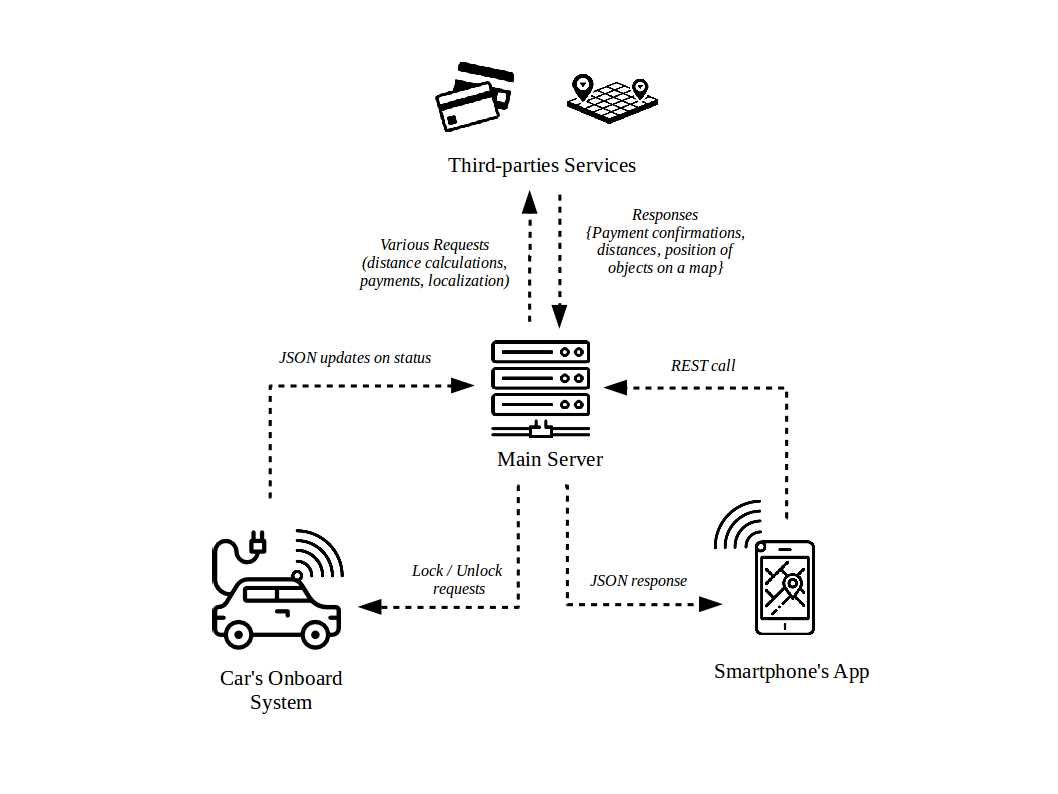
\includegraphics[width=1\textwidth]{proposed_system.png}
	\caption{Description of the proposed system.}
\end{figure}

\subsubsection{App Frontend}
The frontend is a thin app that relies on the smartphone's internet connections in order to work. Almost no operations can be performed with the app alone: all transactions are sent to the main server first, then processed and the result sent back to the app.

The app can be classified as a thin client.

\subsubsection{Centralized Backend}
The backend is the core of the system. Being able to process a lot of parallel operations, it can deal with all the requests coming from che clients ina reasonable amount of time (see Non Functionals Requirements). The backend is based on an MVC architecture and a REST API.

\subsubsection{Car's Onboard system}
The cars are equipped with an onboard system that monitors the status of the car, its location, and can send all the necessary informations to the main server. There won't be direct interactions between the car and the user's app.


